% SPDX-FileCopyrightText: Copyright (c) 2023 Yegor Bugayenko
% SPDX-License-Identifier: MIT

\documentclass{article}

\usepackage[russian]{../../lecture-notes/notes}
\usepackage{svg}
\usepackage{csquotes}
\usepackage{tikz}
  \usetikzlibrary{shadows}

\graphicspath{{../../faces/}}

\newcommand*{\thetitle}{\rus{Враг у ворот}{Enemy at the Gate: AI}}
\newcommand*{\thesubtitle}{\rus{Что защитит наш код от ИИ?}{What is the weapon to defend our code?}}
\newcommand*{\theauthor}{\rus{Егор Бугаенко}{Yegor Bugayenko}}

\newcommand\rus[2]{#1}

\renewcommand\ul[1]{\textcolor{orange}{#1}}

\newcommand\bysora[1]{{\color{gray}\fontsize{12}{12}\selectfont Image by \href{https://sora.chatgpt.com/g/gen_#1}{Sora} \par}}

\begin{document}

\rmfamily

\pptLeft{\rus{29 октября 2025}{October 29th, 2025}}
\pptRight{@yegor256}

\lnPitch{
  \begin{textblock}{8}[1,1](15,15)%
    \raggedleft%
    
\includegraphics[width=.6\linewidth]{arnie.png}\\
    \bysora{01k7xe5sppe8s984jq26grme12}
  \end{textblock}%
  \pptTitle{\thetitle}{\thesubtitle}
  \par
  {\scshape \theauthor}
  \newline
  {\scshape Zerocracy}
}
\newpage
\pagecolor{white}

\lnPitch{
  \pptChapter[\rus{Помехи}{Threats}]{\rus{Что нам всегда мешает?}{What Are the Threats?}}
  \begin{textblock}{8}[1,0](15,2)%
    \raggedleft%
    
\includegraphics[width=.6\linewidth]{coder.png}\\
    \bysora{01k7xjeqxxf9zv3dh82jnpyz7r}
  \end{textblock}}

\lnPitch{
  \pptBanner{\rus{От чего программисты страдают больше всего}{From What We Programmers Suffer Most}:}
  \begin{enumerate}
    \item \rus{Баги}{Bugs}
    \item \rus{Дыры в безопасности}{Security Holes}
    \item \rus{Грязный код}{Dirty Code}
  \end{enumerate}}

\begin{lnSnippet}[bug.java]
int[] nn = {1, 2, 3, 4, 5};
  for (int i = 0; i (*@\textcolor{orange}{<=}@*) nn.length; i++)
    System.out.println(i);
\end{lnSnippet}
\lnPitch{
  \pptSection[1.\rus{Баги}{Bugs}]{\rus{1. Дефекты (они же баги)}{1. Defects a.k.a Bugs}}
  \begin{textblock}{8}[1,1](15,14)%
    \ffinput{bug.java}
  \end{textblock}}

\lnQuote
  [Steve McConnell]
  {steve-mcconnell}
  {\rus{Microsoft обнаруживает около \ul{10–20 дефектов на 1000 строк кода} во время внутреннего тестирования и 0.5 дефектов на 1000 строк кода в выпущенном продукте.}{Microsoft experiences about \ul{10–20 defects per 1000 lines of code} during in-house testing and 0.5 defects per 1000 lines of code in released product.}}
  {mcconnell2004code}

\lnPitch{\pptBanner{\rus{Статистика нескольких современных продуктов}{A Few Open Source Repositories of Our Time}}
  {\ttfamily\small\begin{tabular}{llrr>{\color{orange}}r}
  \toprule
  \rus{Продукт}{Repository} & Stack & KLoC & Issues & I/KLoC \\
  \midrule
  \href{https://github.com/torvalds/kernel}{kernel} & C & 27,300 & 220,600 & 8.1 \\
  \href{https://github.com/tensorflow/tensorflow}{tensorflow} & C++ & 3,600 & 40,200 & 11.2 \\
  \href{https://github.com/flutter/flutter}{flutter} & Dart & 2,100 & 103,000 & 49.0 \\
  \href{https://github.com/rust-lang/rust}{rust} & Rust & 2,100 & 56,500 & 26.9 \\
  \href{https://github.com/microsoft/vscode}{vscode} & TypeScript & 1,500 & 210,000 & 140.0 \\
  \href{https://github.com/apache/spark}{spark} & Java & 1,400 & 53,750 & 38.4 \\
  \href{https://github.com/apache/kafka}{kafka} & Java & 980 & 19,800 & 20.2 \\
  \href{https://github.com/angular/angular}{angular} & TypeScript & 800 & 28,700 & 35.9 \\
  \href{https://github.com/google/guava}{guava} & Java & 346 & 3,600 & 10.4 \\
  \bottomrule
  \end{tabular}}}

\begin{lnSnippet}[loophole.java]
"SELECT * FROM user WHERE name = (*@\textcolor{orange}{'" + x + "'"}@*)
\end{lnSnippet}
\lnPitch{
  \pptSection[2.\rus{Дыры}{Holes}]{\rus{2. Дыры в безопасности}{2. Security Holes}}
  \begin{textblock}{10}[1,1](15,14)%
    \ffinput{loophole.java}
  \end{textblock}}

\lnQuote
  {gary-mcgraw}
  {\rus{Центральный и критический аспект компьютерной \ul{проблемы безопасности} — это проблема программного обеспечения. Дефекты ПО с последствиями для безопасности — включая ошибки реализации, такие как переполнение буфера, и недостатки проектирования, такие как непоследовательная обработка ошибок — обещают быть с нами \ul{годами}.}{A central and critical aspect of the computer \ul{security problem} is a software problem. Software defects with security ramifications—including implementation bugs such as buffer overflows and design flaws such as inconsistent error handling—promise to be with us \ul{for years}.}}
  {mcgraw2006software}

\begin{lnSnippet}[smell.java]
while (!(x = read()))
  if (x = 5 && !(b & 3))
    print( x-- );
    else return;
\end{lnSnippet}
\lnPitch{
  \pptSection[3.\rus{Грязь}{Dirt}]{3. \rus{Сложность, дублирование и smells}{Complexity, Duplication, and Smells}}
  \begin{textblock}{6}[1,1](15,14)%
    \ffinput{smell.java}
  \end{textblock}}

\lnQuote
  {vladimir-khorikov}
  {\rus{Чем \ul{проще} ваше решение, тем \ul{лучше} вы как разработчик. Большинство разработчиков могут написать код, который работает. Создать код, который работает \ul{и} настолько прост, насколько это возможно — вот истинный вызов.}{The \ul{simpler} your solution is, the \ul{better} you are as a software developer. Most software developers can write code that works. Creating code that works \ul{and} is as simple as possible --- that is the true challenge.}}
  {khorikov2015kiss}

\lnQuote
  [Robert C. Martin]
  {robert-martin}
  {\rus{Дублирование — это \ul{главный враг} хорошо спроектированной системы.}{Duplication is the \ul{primary enemy} of a well-designed system.}}
  {martin2008clean}

\lnQuote
  [Mark Seemann]
  {mark-seemann}
  {\rus{Мне нравится, как метафора садоводства подчеркивает действия, которые борются с беспорядком. Точно так же, как вы должны обрезать и пропалывать сад, вы должны рефакторить и погашать \ul{технический долг} в вашей кодовой базе.}{I like the gardening metaphor's emphasis on activities that combat disorder. Just as you must prune and weed a garden, you must refactor and pay off \ul{technical debt} in your code bases.}}
  {seemann2021code}

\lnPitch{
  \pptChapter[LLM]{\rus{Почему сейчас становится хуже?}{Why Now It's Getting Worse?}}
  \begin{textblock}{8}[0,1](1,14)%
    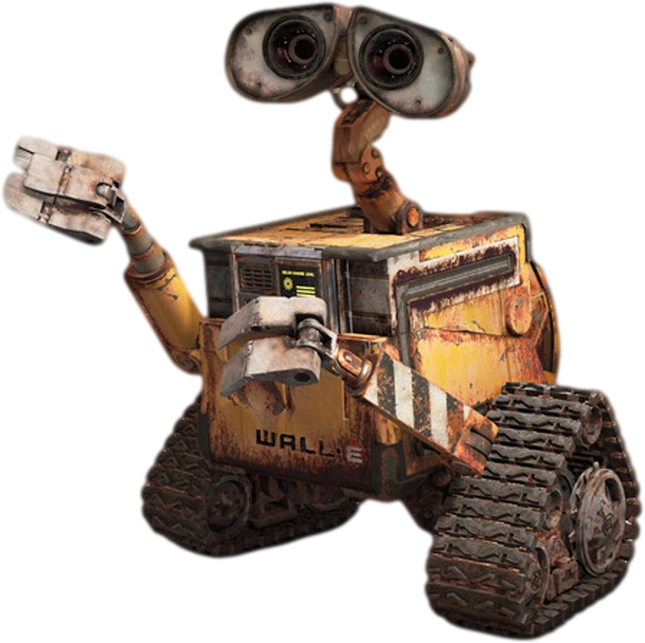
\includegraphics[width=.4\linewidth]{wall-e.png}
  \end{textblock}}

\lnPitch{\pptSection[1.\rus{Качество}{Quality}]{1. \rus{Ложное чувство качества}{False Sense of Quality}}}

\lnQuote
  [Chun Jie Chong]
  {chun-jie-chong}
  {\rus{С точки зрения качества, мы обнаружили, что LLM генерирует голый код, лишенный конструкций защитного программирования, и обычно \ul{более сложный} (на строку кода) по сравнению с кодом, написанным человеком. Фаззинг показал, что код, сгенерированный LLM, более \ul{склонен к зависаниям и сбоям}, чем код, написанный человеком.}{Quality-wise, we found that LLM generates bare-bones code that lacks defensive programming constructs, and is typically \ul{more complex} (per line of code) compared to human-written code. Fuzzing has revealed that LLM-generated code is more \ul{prone to hangs and crashes} than human-written code.}}
  {chong2024artificial}

\lnQuote
  [Altaf Allah Abbassi]
  {altaf-allah-abbassi}
  {\rus{33.54\% изученных образцов продемонстрировали множественные \ul{неэффективности}, указывая на то, что неэффективности в коде, сгенерированном LLM, разнообразны и взаимосвязаны. Наши результаты выявляют \ul{критический пробел} в способности LLM генерировать корректный, оптимизированный и высококачественный код.}{33.54\% of the studied sample exhibited multiple \ul{inefficiencies}, indicating that inefficiencies in LLM-generated code are diverse and interconnected. Our findings highlight a \ul{critical gap} in LLMs' capability to generate correct, optimized, and high-quality code.}}
  {abbassi2025taxonomy}

\lnQuote
  [Adam Alami]
  {adam-alami}
  {\rus{Внедрение LLM в социальную систему ревью кода вызывает \ul{нарушение} присущей социальной динамики процесса и переход \ul{ответственности} от индивидуальной к коллективной.}{Introduction of an LLM into the social system of code review causes a \ul{disruption} to the inherent social dynamics of the process and to the transition of \ul{accountability} from individual to collective.}}
  {alami2025accountability}

\lnPitch{\pptSection[2.\rus{Влияние}{Influence}]{2. \rus{Дурное влияние}{Bad Influence}}}

\lnQuote
  [Xuanhua Shi]
  {xuanhua-shi}
  {\rus{Стиль кодирования человеческого кода может быть подвержен влиянию LLM: они могут не только отражать существующие нормы, но и тонко изменять их, постепенно подталкивая разработчиков к большему стилистическому соответствию с \ul{конвенциями, предпочитаемыми LLM}.}{The coding style of human-written code may be influenced by LLMs: they may not only mirror existing norms but also subtly reshape them, gradually pushing human developers toward greater stylistic alignment with \ul{LLM-preferred conventions}.}}
  {xu2025transformed}

\lnPitch{\pptSection[3.\rus{Утечки}{Leakage}]{\rus{3. Случайная утечка данных}{3. Accidental Leakage of Data}}}

\lnPitch{
  \includesvg[height=1in]{gemini.svg}
  \par
  \pptPic{.9}{gemini.png}
  \par
  {\scriptsize\url{https://support.google.com/gemini/answer/13594961}}}

\lnPitch{
  
\includegraphics[height=1in]{giga-logo.png}
  \par
  \pptPic{.9}{giga.png}
  \par
  {\scriptsize\url{https://developers.sber.ru/docs/ru/policies/gigachat-agreement/beta}}}

\lnPitch{\pptSection[4.\rus{Начальство}{Bosses}]{4. \rus{Давление менеджмента}{Management Pressure}}}

\lnPitch{
  \pptBanner{\rus{Недавний опрос в моем Telegram канале}{Recently Asked in My Telegram Channel}:}
  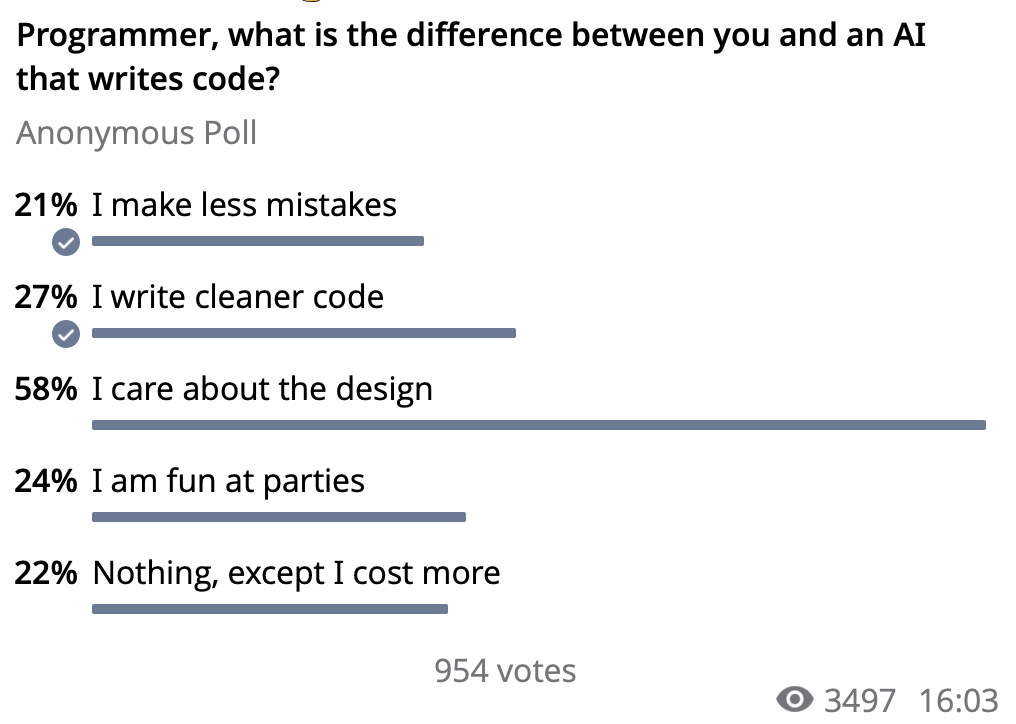
\includegraphics[width=.5\linewidth]{poll.png}
  \par
  {\scriptsize\url{https://t.me/yegor256news/1721}}}

\lnPitch{\pptChapter[Defense]{\rus{Как мы можем защититься?}{How Can We Defend Ourselves?}}}

\lnPitch{
  \pptBanner{\rus{Наше оружие против ИИ}{Our Ammunition Against LLM}:}
  \begin{enumerate}
    \item \rus{Ревью кода}{Code Reviews}
    \item \rus{Автоматизированные тесты}{Automated Tests}
    \item \rus{Стандарты качества}{Quality Standards}
    \item \rus{Контроль стиля}{Style Checkers}
    \item \rus{Описание архитектуры}{Written Architecture}
  \end{enumerate}}

\lnPitch{
  \pptSection[1.\rus{Ревью}{Reviews}]{1. \rus{Ревью кода малыми порциями}{Reviews in Small Pull Requests}}
  \begin{textblock}{8}[1,1](15,14)%
    \raggedleft%
    
\includegraphics[width=.45\linewidth]{glass.png}\\
    \bysora{01k815cxgzfshswvj9mqv9whtg}
  \end{textblock}}

\lnQuote
  [\nospell{Caitlin Sadowski}]
  {caitlin-sadowski}
  {\rus{Корреляция между \ul{размером изменения} и \ul{качеством ревью} признается Google, и разработчикам настоятельно рекомендуется вносить небольшие, инкрементальные изменения (за исключением больших удалений и автоматизированного рефакторинга).}{A correlation between \ul{change size} and \ul{review quality} is acknowledged by Google and developers are strongly encouraged to make small, incremental changes (with the exception of large deletions and automated refactoring).}}
  {sadowski2018modern}

\lnPitch{
  \begin{multicols}{2}
  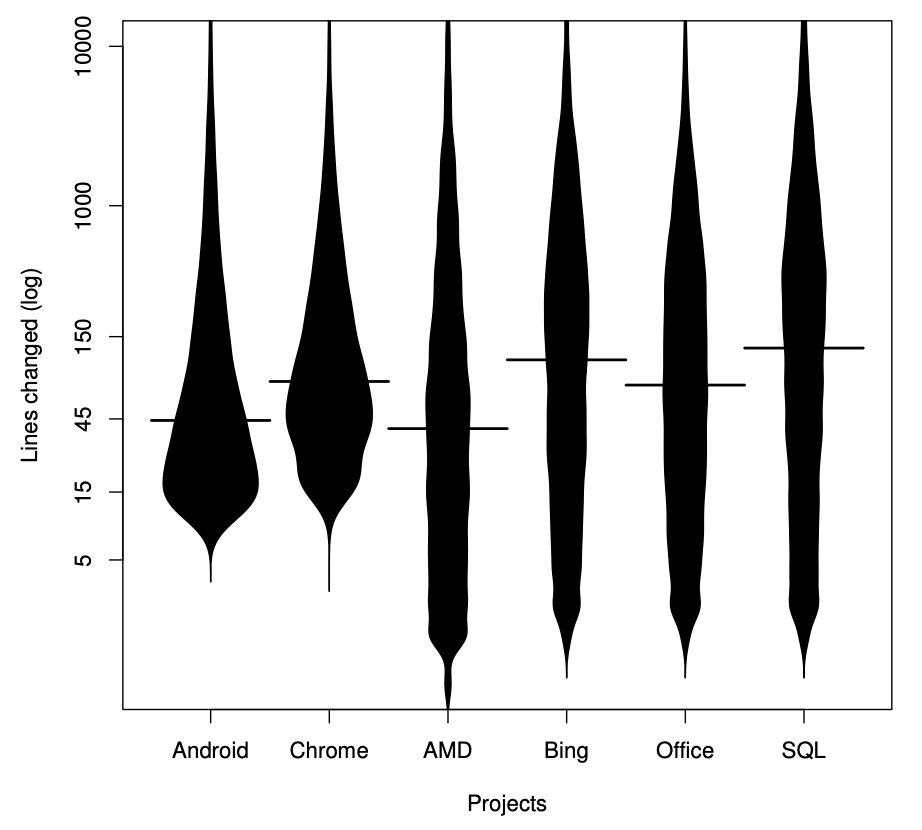
\includegraphics[width=.7\linewidth]{lines-per-pr.png}\par
  \lnSource{rigby2013convergent}
  \par\columnbreak\par
  \enquote{Both Android and AMD have a median change size of 44 lines. This median change size is larger than Apache, \ul{25 lines}, and Linux, \ul{32 lines}, but much smaller than Lucent where the number of non-comment lines changed is \ul{263 lines}. Bing, Chrome’s median change is \ul{78 lines} and includes 5 files.}
  \end{multicols}}

\lnPitch{
  \pptSection[2.\rus{Тесты}{Tests}]{2. \rus{Контроль покрытия тестами}{Test Coverage Control}}
  \begin{textblock}{8}[1,1](15,14)%
    \raggedleft%
    
\includegraphics[width=.45\linewidth]{brick.png}\\
    \bysora{01k815qsb1e6csjmmbxsdqexjv}
  \end{textblock}}

\lnQuote
  [Goran Petrovi{\'c}]
  {goran-petrovic}
  {\rus{Google \ul{не применяет принудительно} никаких порогов покрытия кода по всей кодовой базе. Проекты (или группы проектов) свободны определять свои собственные пороги и цели. Многие проекты подключаются к централизованной добровольной системе оповещения, которая определяет \ul{пять уровней} порогов покрытия кода.}{Google \ul{does not enforce} any code coverage thresholds across the entire codebase. Projects (or groups of projects) are free to define their own thresholds and goals. Many projects opt-into a centralized voluntary alerting system that defines \ul{five levels} of code coverage thresholds.}}
  {ivankovi2019}

\lnPitch{
  \pptBanner{Code Coverage Threshold Levels in Google}
  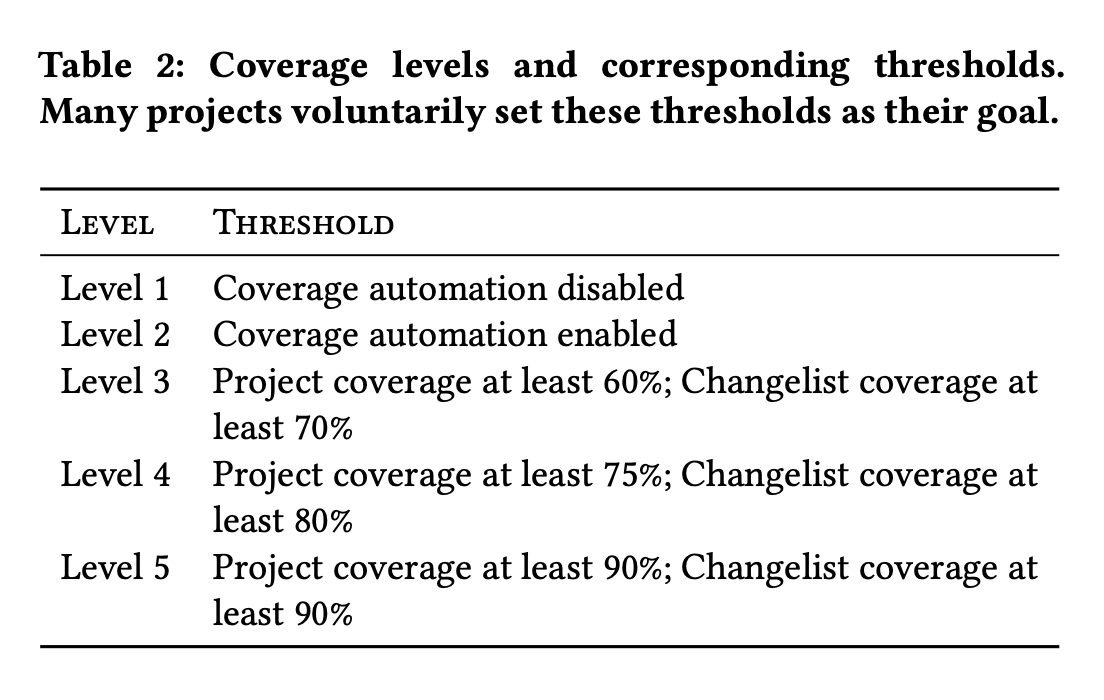
\includegraphics[width=.6\textwidth]{levels.png}
  \lnSource{ivankovi2019}}

\lnPitch{
  \pptSection[3.\rus{Стандарты}{Standards}]{3. \rus{Стандарты кодирования}{Coding Standards}}
  \begin{textblock}{8}[1,1](15,14)%
    \raggedleft%
    
\includegraphics[width=.45\linewidth]{manifest.png}\\
    \bysora{01k81bvz5we3cbmenbcsef59nr}
  \end{textblock}}

\lnPitch{
  \pptPic{.9}{karpathy.png}
  {\scriptsize \url{https://x.com/karpathy/status/1617979122625712128}\par}}

\lnPitch{
  \pptBanner{Our \enquote{Agent Coding Manifest}}
  \pptPic{.7}{prompt.png}
  {\small\url{https://github.com/yegor256/prompt}}}

\lnPitch{
  \pptBanner{Leaked System Prompts:}
  \texttt{\href{https://github.com/asgeirtj/system_prompts_leaks}{asgeirtj/system\_prompts\_leaks}}}

\lnPitch{
  \pptSection[4.\rus{Стиль}{Style}]{4. \rus{Контроль стиля}{Style Checkers}}
  \begin{textblock}{8}[1,1](14,14)%
    \raggedleft%
    
\includegraphics[width=.5\linewidth]{girl.png}\\
    \bysora{01k7xmxhcfedwr5qa3wekfegtm}
  \end{textblock}}

\lnPitch{
  \pptBanner{\rus{Несколько популярных контролёров стиля}{Some Popular Style Checkers}:}
  \begin{itemize}
    \setlength\itemsep{0em}
    \item \href{https://eslint.org/}{ESLint} \rus{для}{for} JavaScript
    \item \href{https://clang.llvm.org/extra/clang-tidy/}{Clang-Tidy} \rus{для}{for} C++
    \item \href{https://github.com/pylint-dev/pylint}{Pylint} \rus{для}{for} Python
    \item \href{https://github.com/rubocop/rubocop}{Rubocop} \rus{для}{for} Ruby
    \item \href{https://github.com/squizlabs/PHP_CodeSniffer}{PHP\_CodeSniffer} \rus{для}{for} PHP
    \item \href{https://github.com/rust-lang/rustfmt}{rustfmt} \rus{для}{for} Rust
    \item \href{https://www.qulice.com}{Qulice} \rus{для}{for} Java: \href{https://checkstyle.sourceforge.io/}{Checkstyle} + \href{https://pmd.github.io/}{PMD}
  \end{itemize}}

\lnPitch{
  \pptBanner{\rus{Сколько правил в контролёрах стиля}{How Many Rules in Style Checkers}:}
  \begin{itemize}
    \setlength\itemsep{0em}
    \item 690+ \rus{в}{in} Clang-Tidy (C++)
    \item 550+ \rus{в}{in} Rubocop (Ruby)
    \item 400+ \rus{в}{in} PMD (Java)
    \item 130+ \rus{в}{in} Checkstyle (Java)
    \item 120+ \rus{в}{in} Pylint (Python)
  \end{itemize}
  \par{\small\rus{Некоторые/большинство правил не только проверяют стиль, но и находят баги.}{Some/most of the rules not only check style, but also find bugs.}\par}}

\lnPitch{
  \pptBanner{\rus{Экзотические контролёры стиля}{Some Exotic Style Checkers}:}
  \begin{itemize}
    \setlength\itemsep{0em}
    \item \href{https://github.com/koalaman/shellcheck}{Shellcheck} \rus{для}{for} Bash
    \item \href{https://github.com/hadolint/hadolint}{Hadolint} \rus{для}{for} Dockerfile
    \item \href{https://github.com/markdownlint/markdownlint}{markdownlint} \rus{для}{for} Markdown
    \item \href{https://github.com/mrtazz/checkmake}{Checkmake} \rus{для}{for} Makefile
    \item \href{https://github.com/yegor256/xcop}{xcop} \rus{для}{for} XML
  \end{itemize}}

\lnPitch{
  \pptSection[5.\rus{Архитектура}{Architecture}]{5. \rus{Описание архитектуры}{Written Architecture}}
  \begin{textblock}{8}[1,1](15,14)%
    \raggedleft%
    
\includegraphics[width=.45\linewidth]{kid.png}\\
    \bysora{01k81dd498eg8st2y5p19xfm59}
  \end{textblock}}

\begin{lnSnippet}[foo.java]
class Foo {
  int get_content(char* path) {
    if cant_read() (*@\textcolor{orange}{return -1}@*);
    // do the rest
    (*@\textcolor{orange}{return 0}@*);
  }
}
\end{lnSnippet}
\begin{lnSnippet}[bar.java]
class Bar {
  void store_it() {
    if cant_save()
      (*@\textcolor{orange}{throw}@*) "Can't save file"
    // do the rest
  }
}
\end{lnSnippet}
\lnPitch{
  \pptBanner{\rus{Некоторые баги на уровне дизайна}{Some Bugs Are at the Design Level}:}
  \begin{pptWide}{2}
  \rus{Код ошибки}{Error code}:\par
  {\small\ffinput{foo.java}}
  \par\columnbreak\par
  \rus{Исключение}{Exception}:\par
  {\small\ffinput{bar.java}}
  \end{pptWide}}

\lnQuote
  [Simon Weber]
  {simon-weber}
  {\rus{В ходе исследования было обнаружено, что \ul{популярные} проекты имеют \ul{более объемные README} (медиана 2 килобайта против 500 байт). Также 95\% популярных проектов имеют непустые README, по сравнению с только 65\% непопулярных проектов.}{Upon investigation, \ul{popular} projects were found to have \ul{larger READMEs} (median 2 kilobytes vs. 500 bytes). Also, 95\% of popular projects have nonempty READMEs, compared to only 65\% of unpopular projects.}}
  {weber2014makes}

\lnPitch{
  \pptBanner{\rus{ArchUnit устанавливает ограничения}{ArchUnit Sets Restrictions}}
  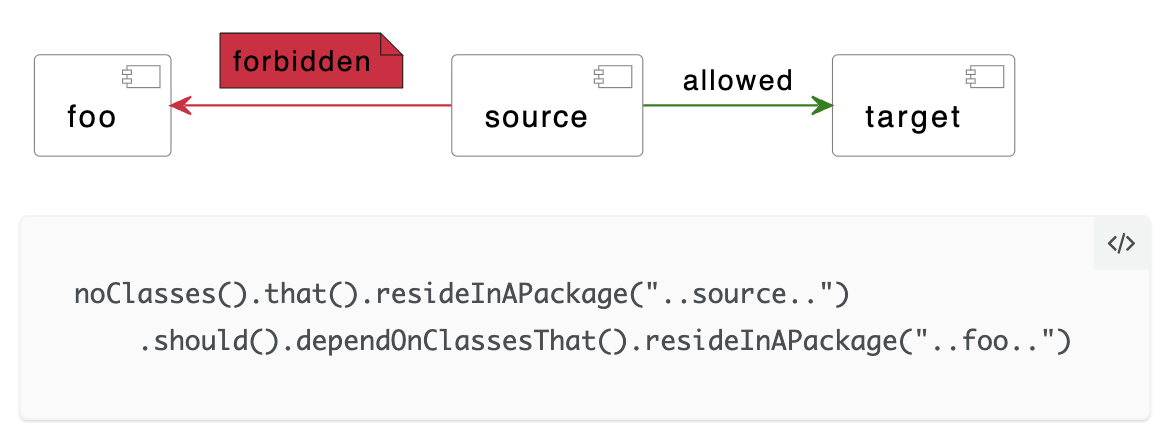
\includegraphics[width=.8\linewidth]{archunit.png}
  \par
  {\scriptsize\url{https://www.archunit.org/}}}

\lnPitch{
  \pptBanner{\rus{Вывод}{Conclusion}:}
  \enquote{\rus{ИИ помогает как нам, так и нашим врагам.}{AI helps us, but it also helps our enemies.}}}

\lnPitch{
  \pptBanner{\rus{Вопросы?}{Questions?}}\par
  \qrcode[height=12em]{https://t.me/yegor256news}}

\end{document}
